\documentclass[10pt]{article}
\usepackage[fontsize=10pt]{fontsize}

\usepackage[margin=0.5in]{geometry} 
\usepackage{amsmath,amsthm,amssymb, graphicx, multicol, array, txfonts}
\usepackage{bbm}
\usepackage{hyperref}
\hypersetup{
    colorlinks=true,
    linkcolor=blue,
    filecolor=magenta,      
    urlcolor=cyan,
    pdftitle={Overleaf Example},
    pdfpagemode=FullScreen,
    }

\urlstyle{same}


\newcommand{\N}{\mathbb{N}}
\newcommand{\Z}{\mathbb{Z}}
\setcounter{secnumdepth}{0}
\setlength\parindent{0pt}

 
\newenvironment{problem}[2][Problem]{\begin{trivlist}
\item[\hskip \labelsep {\bfseries #1}\hskip \labelsep {\bfseries #2.}]}{\end{trivlist}}

\newenvironment{prelim}[2][Preliminaries]{\begin{trivlist}
\item[\hskip \labelsep {\bfseries #1}\hskip \labelsep {\bfseries #2}]}{\end{trivlist}}
    
\begin{document}
 
\title{6.S091: Problem Set 3}
\author{Suyeol Yun\\
syyun@mit.edu}
\maketitle
 
\section{Problem 1: Constructing Minimal I-MAPs [5 points]}
* Code is available at \url{https://github.com/syyunn/6.S091/blob/main/pset3/pb1.py}

\subsection{(a)} 
1. Draw $\mathcal{G}_{\pi_a}$\\

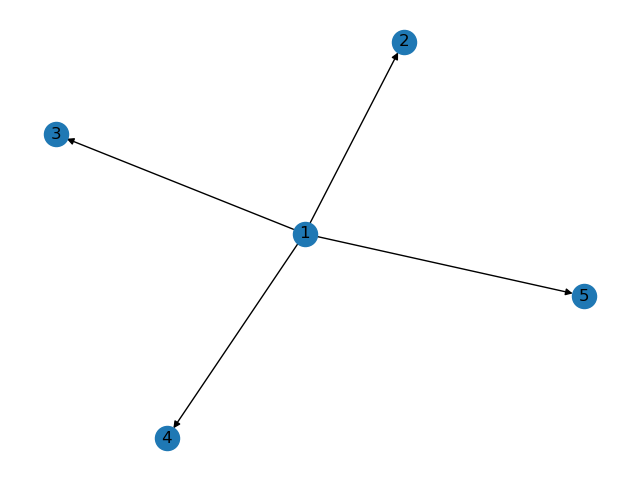
\includegraphics{images/pb1a.png}

2. Draw $\mathcal{G}_{\pi_b}$\\

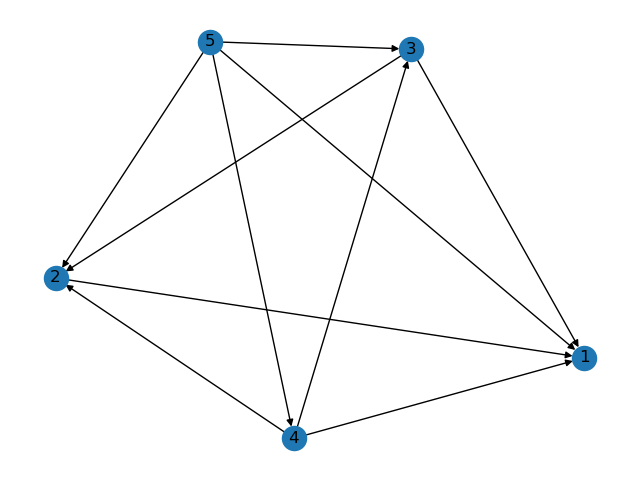
\includegraphics{images/pb1b.png}

3. Draw $\mathcal{G}_{\pi_c}$\\

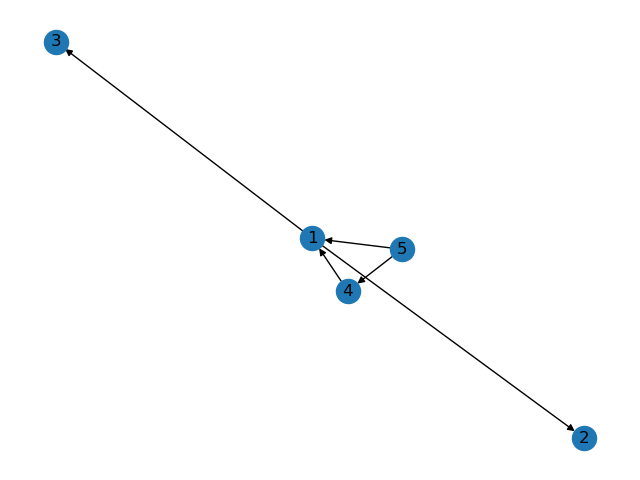
\includegraphics{images/pb1c.png}

\subsection{(b)}
We can transform  $\mathcal{G}_{\pi_a}$ into $\mathcal{G}_{\pi_c}$ by the Chickering sequence (Add $5 \rightarrow 4$, Reverse $1\rightarrow 5$, then Reverse $1\rightarrow 4$).

\section{Problem 3}
* Code is available at \url{https://github.com/syyunn/6.S091/blob/main/pset3/search_mec.py}

\subsection{(a)}
$\text { starting\_dag2 and 3 }$ both have $4$ neighbors. 
\subsection{(b)}
1. $\text { starting\_dag2}$ has the shortest path of length $1$.\\
2. $\text { starting\_dag3}$ has the shortest path of length $3$.
\end{document}
